\section{GUI Design}
\paragraph{WPF Ressourcen}
Mit WPF Ressourcen kann man nützliche Objekte (Image, Brushes, Styles, Templates etc.) zentral definieren und wiederverwenden.


\paragraph{Physikalische Ressourcen} In den File Properties kann man eine Datei als WPF-Ressource deklarieren welche dann in die Binärdatei einkompiliert werden. Zugegriffen kann dann mittels Resource-Key (relativer Pfadname).
\begin{lstlisting}[language=xml]
<Image Source="Desert.jpg" />
\end{lstlisting}


\paragraph{Resource}
\begin{itemize}
    \item Beliebige Objekte in XAML können als Ressource definiert werden
    \item Wird mit dem Key-Attribut aus dem x-Namespace benannt
\end{itemize}
\begin{lstlisting}[language=xml]
<Application.Resources>
    <SolidColorBrush x:Key ="MyButtonBackground" Color="#EEEEEE" />
</Application.Resources>
\end{lstlisting}
Unter diesem Key sind Ressourcen dann auch ansprechbar
\begin{lstlisting}[language=xml]
<Button ...>
  <Button.Background>
    <StaticResource ResourceKey="MyBg" />
  </Button.Background>
</Button>

<Button Background="{StaticResource MyButtonBackground}" Content="Save" />
\end{lstlisting}


\paragraph{ResourceDictionary} 
\begin{itemize}
    \item Behälter um Ressourcen zu speichern
    \item Indexiert nach Ressourcen-Namen (\verb+x:Key+)
    \item In mehrere Elementen out-of-the-box verfügbar
    \begin{itemize}
        \item Application.Resources
        \item Window.Resources
        \item Button.Resources
        \item Label.Resources
    \end{itemize}
    \item Schont die Ressourcen (Mehrfachverwendung)
    \item Die Reihenfolge im XAML ist wichtig
\end{itemize}



\paragraph{FindResource} Mit der Methode \verb+FrameworkElement.FindResources+  können Zugriffe auf XAML Resourcen im Code-behind gemacht werden.
\begin{lstlisting}
var okText = (string)FindResource("OkText");
var bgBrush = FindResource("DarkBrush") as Brush;
\end{lstlisting}

\subsubsection{Zugriff}
\begin{enumerate}
    \item Key wird im Element und in allen Parent-Nodes gesucht.
    \item Key wird in Application.Resources gesucht.
    \item Key wird in System-Ressourcen gesucht.
\end{enumerate}

% \paragraph{System Ressources} Auf Ressourcen in Namespace \verb+System.Windows+ kann man mittels statischer Properties zugegriffen werden. Dazu gehören: \verb+SystemColors+, \verb+SystemFonts+ und \verb+SystemParamters+.
% \begin{lstlisting}[language=xml]
% StaticResource="{StaticResource[name]}"
% \end{lstlisting}
% Die Statische Bindung macht CompileTime Check und findet Fehler früh.
% \begin{lstlisting}[language=xml]
% DynamicResource="{DynamicResource[name]}"
% \end{lstlisting}
% Anstelle von \verb+[name]+ steht der Key der Ressource
% In der Dynamische Bindung wird ein RuntimeCheck gemacht und lässt dynamisch erzeugte und geladene Ressourcen zu. Beim Static Binding wird bei Objektkonstruktion ausgewertet, beim Dynamic Binding einmal pro Zugriff.

\paragraph{Static vs DynamicResource}
\begin{lstlisting}[language=xaml]
<Button ... Background="{StaticResource MyBg}" />
<Button ... Background="{DynamicResource MyBg}" />
\end{lstlisting}

\textbf{Static Resources}
\begin{itemize}
    \item Anstelle von \code{name} steht der Key der Ressouce
    \item Statische Bindung an Ressource $\Longrightarrow$ 1-malig beim Laden
    \item Compile Time Check $\Longrightarrow$ findet den Fehler früh 
\end{itemize}
\textbf{Dynamic Resources}
\begin{itemize}
    \item Anstelle von \code{name} steht der Key der Ressouce
    \item Dynamische Bindung (bei jedem Zugriff)
    \item Runtime Check $\Longrightarrow$ lässt dynamisch erzeuge Ressourcen zu
\end{itemize}


\paragraph{Eigene ResourceDictionaries}
\begin{itemize}
    \item Separates xaml-File
    \item In andere ResourceDictionaries einbindbar
    \item XML-Root-Node ist <ResourceDictionary>
\end{itemize}
\begin{lstlisting}[language=xml]
<ResourceDictionary xmlns="http://schemas.microsoft.com/winfx/2006/xaml/presentation" xmlns:x="http://schemas.microsoft.com/winfx/2006/xaml" xmlns:local="clr-namespace:Microsoft.FamilyShow"> 

  <!-- place your resources here --> 
  
</ResourceDictionary> 
\end{lstlisting}

Zum Einbinden muss ein \code{MergedDictionary} verwendet werden:
\begin{lstlisting}[language=xml]
<Application.Resources>
  <ResourceDictionary>
    <!– you can mix resources and merged dictionaries -->
    <SolidColorBrush x:Key ="MyButtonBackground" Color="#EEEEEE" />
   
    <ResourceDictionary.MergedDictionaries>
      <!– just list your external resource dictionaries, here --> 
      <!– (the order is important!) -->
      <ResourceDictionary Source="Colors.xaml"/>
      <ResourceDictionary Source="Brushes.xaml"/>
      </ResourceDictionary.MergedDictionaries>
    </ResourceDictionary>
</Application.Resources> 
\end{lstlisting}

\section{Externe Resources einbinden}
Für das Einbinden von externen Ressourcen, z.B Bilder, gibt es verschiedene Möglichkeiten.
\paragraph{Gleiche Assembly}
Einbinden einer Ressource von derselben Assembly:
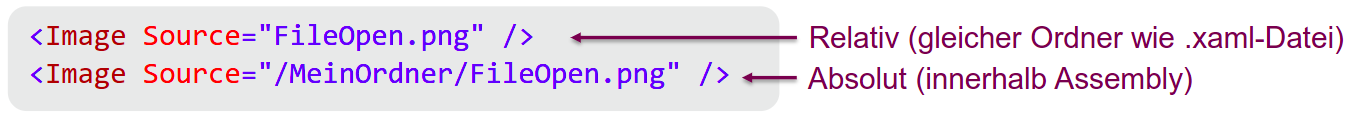
\includegraphics[scale=0.18]{img/resource-same-assembly.png}

\paragraph{Externe Assembly}
Einbinden einer Ressourcen von einer anderen Assembly:
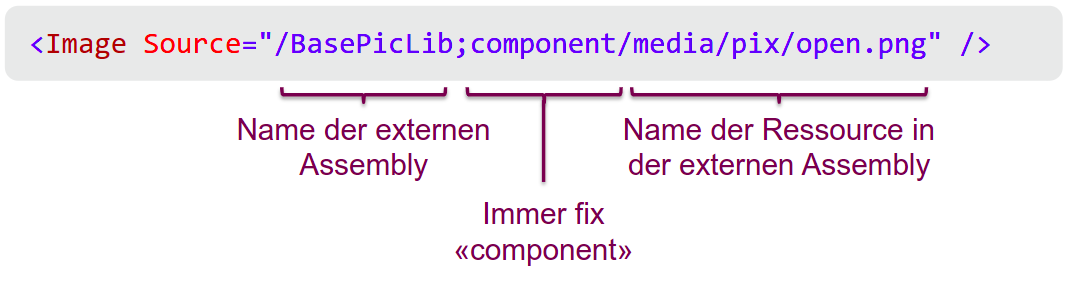
\includegraphics[scale=0.22]{img/ressource-other-assembly.png}

\paragraph{Absolute Angabe}
Sollte nicht verwendet werden, da bei jeder Umgebung anders (zu starke Bindung).

\paragraph{PackageURI}
Es wird ein PackageURI verwendet, welcher spezifiziert, 
\begin{lstlisting}[language=xml]
<!--Relativ zum aktuellen Ordner--!>
<Image Source="pack://siteOfOrigin:,,,/media/pix/open.png" />
<!--Relativ zur Assembly--!>
<Image Source="pack://application:,,,/media/pix/open.png" /> 
\end{lstlisting}

\paragraph{Zugriff aus statische Werte (z.B System Ressourcen)}
Es gibt verschiedene System-Ressourcen:
\begin{itemize}
    \item SystemColors - z.B SystemColors.WindowTextColor
    \item SystemFonts - z.B SystemFonts.MenuFontFamily
    \item SystemParameters - z.B SystemParameters.PrimaryScreenWidth
\end{itemize}
\begin{lstlisting}
<Button Background="{x:Static SystemColors.ControlBrush}" Content="Save" /> 
<TextBox FontFamily="{x:Static SystemFonts.MenuFontFamily}" > ... 
\end{lstlisting}

\section{Styles}
Das Aussehen sollte ausschliesslich über Styles und Templates definieren werden! 
\subsubsection{implizit (typspezifisch)}
\begin{itemize}
    \item \textbf{x:Key} wird weggelassen
    \item \code{TargetType="Button"} benutzen
    \item Klassenname (\code{Button.Foreground}) kann weggelassen werden
    \item Style gilt für alle Elemente wenn man den Key weglässt
\end{itemize}
\begin{lstlisting}[language=xml]
<!-- App.xaml -->
<Application x:Class="ModernUi.App"
             xmlns="http://schemas.microsoft.com/winfx/2006/xaml/presentation"
             xmlns:x="http://schemas.microsoft.com/winfx/2006/xaml"
             xmlns:local="clr-namespace:ModernUi"
             StartupUri="MainWindow.xaml">
    <Application.Resources>
        <ResourceDictionary Source="style.xaml"></ResourceDictionary>
    </Application.Resources>
</Application>
\end{lstlisting}
\begin{lstlisting}[language=xml]
<!-- Style.xaml -->
<Window.Resources>
    <!-- benannten Style als Basis benutzen -->
    <Style x:Key="DefaultButtonStyle" TargetType="Button">
      <Setter Property="BorderThickness" Value="1" />
      <Setter Property="BorderBrush" Value="Black" />
      <Setter Property="Background" Value="Transparent" />
      <Setter Property="Foreground" Value="Black" />
      <Setter Property="FontFamily" Value="Segoe UI" />
      <Setter Property="Margin" Value="2" />
      <Setter Property="Padding" Value="10 2 10 2" />
      <Setter Property="FontSize" Value="13" />
    </Style>
    
    <!-- Den obigen benannten Style erben und auf alle Buttons anwenden -->
    <Style TargetType="Button" BasedOn="{StaticResource DefaultButtonStyle}"> </Style>
    
    <!-- fuer den Help Button noch einen abgeleiteten Style definieren --> 
    <Style x:Key="MyHelpButtonStyle" TargetType="Button"
           BasedOn="{StaticResource DefaultButtonStyle}">
      <Setter Property="Foreground" Value="Gray" />
      <Setter Property="BorderBrush" Value="Gray" />
    </Style>
</Window.Resources>
\end{lstlisting}
\begin{lstlisting}[language=xml]
<!-- Window.xaml -->
<Button Style="{StaticResource DefaultButtonStyle}" Content="OK" />
\end{lstlisting}

\subsubsection{explizit}
Haben einen expliziten \textbf{x:key}
\begin{lstlisting}[language=xml]
<Style x:Key="MyButtonStyle">
    <Setter Property="Button.Foreground" Value="#000000" />
    <Setter Property="Button.Background" Value="#FFFFFF" />
    <!-- auch komplexes möglich -->
    <Setter Property="Button.Background">
        <Setter.Value>
            <LinearGradientBrush StartPoint="0,0" EndPoint="0,1">
                <GradientStop Offset="0" Color="#dddddd"></GradientStop>
                <GradientStop Offset="0.5" Color="#F0F0F0"></GradientStop>
                <GradientStop Offset="1" Color="#dddddd"></GradientStop>
            </LinearGradientBrush>
        </Setter.Value>
    </Setter>
</Style>
\end{lstlisting}
Verwenden mit:
\begin{lstlisting}[language=xml]
<Button Style="{StaticResource MyButtonStyle}" Content="Cancel" />
\end{lstlisting}



\subsubsection{Styles kombinieren}
\begin{itemize}
    \item Styles können abgeleitet werden
    \item Styles mit Inline Eigenschaften kombinierbar
\end{itemize}
\begin{lstlisting}[language=xml]
<Style x:Key="DangerButtonStyle" 
      TargetType="Button" 
      BasedOn="{StaticResource MyButtonStyle}"> 
  <Setter Property="Background" Value="Red" /> 
</Style> 
\end{lstlisting}

\subsection{Control Templates}
\begin{itemize}
    \item Legt die Inhaltsdarstellung eines Controls fest
    \item Für alle visuellen Control-Typen vorgegeben
    \item Jede Windows Version hat passendes Theme
    \item Legt Standard-Aussehen eines XAML Controls fest
\end{itemize}
\paragraph{Template Binding}
\begin{itemize}
    \item Markup Extension, die eine verkürzte Form des Data Bindings anbietet
    \item Nur innerhalb Control Template
    \item Kann Wert einer Dependency Property im Control (oder Style) abrufen
\end{itemize}
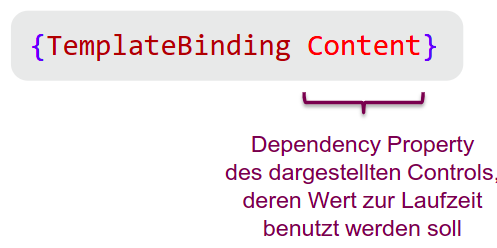
\includegraphics[scale=0.3]{img/template-binding.png}

\subsection{Style Trigger}
Style anhand unterschiedlicher UI-Zustände anpassen
\begin{lstlisting}[language=xml]
<Style x:Key="MyButtonStyle" TargetType="Button"> 
  <Setter Property="Background" Value="White" /> 
  <Setter Property="Foreground" Value="Black" /> 
  <Setter Property="Cursor" Value="Hand" /> 
  <Style.Triggers> 
    <Trigger Property="IsMouseOver" Value="True"> 
      <Setter Property="Background" Value="#2672EC" /> 
      <Setter Property="Foreground" Value="White" /> 
    </Trigger> 
  </Style.Triggers> 
</Style> 
\end{lstlisting}


\subsection{Data Trigger}
(in \code{Style.Triggers} eingebunden, wie vorher. Beispiel: Style ist für ListBoxItem, rote Schrift wenn nicht mehr an Lager (\code{InStock == 0})
\begin{lstlisting}
<DataTrigger Binding="{Binding InStock}" Value="0">
    <Setter Property="Foreground" Value="Red" />
</DataTrigger>
\end{lstlisting}

\subsection{Standardverhalten Überschreiben}
\begin{lstlisting}[language=xml]
<Style x:Key="BaseButtonStyle" TargetType="{x:Type ButtonBase}"> 
  ... 
  <Setter Property="Template"> 
    <Setter.Value> 
      <ControlTemplate.Triggers> 
        ... 
        <Trigger Property="IsMouseOver" Value="true"> 
          <Setter Property="Background" Value="{StaticResource Button.MouseOver.Background}" TargetName="border" /> 
          <Setter Property="BorderBrush" Value="{StaticResource Button.MouseOver.Border}" TargetName="border" /> 
        </Trigger> 
        ... 
      </ControlTemplate.Triggers> 
    </Setter.Value> 
  </Setter> 
</Style>
\end{lstlisting}

\subsection{Transformationen}
\subsubsection{2D Transformation}
\begin{lstlisting}[language=xml]
<ScaleTransform ScaleX="1.5" ScaleY="1.5" />
<RotateTransform Angle="45" CenterX="30" CenterY="12" /> 
<SkewTransform AngleX="-35" AngleY="9" />
<TranslateTransform X="40" Y="-10" /> 
\end{lstlisting}
\subsubsection{Transformationen in Styles}
Normal via Style Setter zu bewerkstelligen
\begin{lstlisting}[language=xml]
<Setter Property="RenderTransform"> 
  <Setter.Value> 
    <RotateTransform Angle="3"></RotateTransform> 
  </Setter.Value> 
</Setter> 
\end{lstlisting}
Un um den Ursprungspunkt/Angelpunkt der Transformation anzugeben
\begin{lstlisting}[language=xml]
<Setter Property="RenderTransformOrigin" Value="0.5,0.5"/> 
\end{lstlisting}
